\documentclass[10pt]{article}
\usepackage[T1]{fontenc}
\usepackage{lmodern,amsmath,amssymb,graphicx,hyperref}
\usepackage[margin=.74in]{geometry}
\setlength{\parindent}{0pt}\setlength{\parskip}{7pt}
\begin{document}
\begin{center}{\Large Actual zeroth-mode support for every positive cutoff}\\[4pt]
Local continuation --- 15 November 2026\end{center}
\textbf{Result.} The actual matching-port zeroth-mode right coefficient remains
exactly one for every $k>0$, extending the preceding $k=1$ result. The left
factor remains the constant polynomial one. The finite set requiring nonzero
support on both sides is therefore all $2^u$ residue labels. This rules out
zero-detection pruning of this actual zeroth layer, without assuming positive
anchor multiplicities [pcc:unverified].

\textbf{Actual source identities.} Let $D(H,Z)$ be the constructed denomRows
and $N(Z)$ the actual matching-port rowNumerator at $t=-2^i$. The proof derives
\[
 [H^0Z^0]D=1,\qquad [Z^0]N=0,\qquad [Z^1]N=1.
\]
For the actual finite geometric sum $G_k=\sum_{s<k}(1-D)^s$, composition of
the two constant-coefficient ring maps gives
\[
 [H^0Z^0]G_k=\sum_{s<k}(1-1)^s=1 \qquad(k>0).
\]
Consequently $[Z^1]([H^0](NG_k))=1$. The theorem applies to the actual
polyRight expression with zeroth moment index, not an abstract favorable
factor or a declared capacity [pcc:unverified].

\textbf{Support witnesses and count.} Under $u\le a$, $i\le a$ and arbitrary
natural multiplicities, each $r<2^u$ has matching class ports satisfying
\[
 L_{r,(r,0)}=1,\qquad [Z^1]R_{(r,0),r}=1.
\]
Define $\mathcal A_{0,k}$ to require both an actual nonzero left factor and an
actual nonzero right factor. The witnesses prove
\[
 \mathcal A_{0,k}=\{0,\ldots,2^u-1\},\qquad
 |\mathcal A_{0,k}|=2^u \quad(k>0).
\]
The statement does not assume linear independence and does not claim a lower
bound for arbitrary alternate factorizations or algorithms [pcc:unverified].

\textbf{Evidence.} Accepted076 contains371 local theorem statements including
parent367, four new. Receipt039 pins exact source, raw compiler output and
exit0 with no warnings. Its central dependency print is standard. Accepted078 contains376 statements including371, five new; it exits0 with
no warnings. Receipt040 separately pins the joint active-set count and generic
control below; they are not inferred from076. All evidence remains local,
unsigned and defaultnot\_covered, outside shared Transport53/57/fresh
[pcc:unverified].

\textbf{Sources and retained failure.} The actual formulas come from pinned
OrientationCompact, Higher, Node and Jet sources, with standard Mathlib
constant-coefficient homomorphisms, finite sums and coefficient products.
The primary creation and prior source reviews remain unchanged. KB tools and
wrapper executable were unavailable; exact repository/primary fallback was
used. Failed075 and all compiler logs are retained; its evalRingHom interface
failure is not a mathematical counterexample [pcc:unverified].
\newpage
\begin{center}{\Large A separate parity control and the next actual test}\end{center}
\textbf{Exact generic control.} Over $\mathbb Q[H]$, the source proves
\[
 (1-cH)(1+cH)=1-c^2H^2.
\]
For every natural cutoff $k$ and odd index $2b+1$ it also proves
\[
 [H^{2b+1}]\sum_{s<k}(c^2H^2)^s=0.
\]
The proof expands the actual finite sum; each summand has only even degree.
These are standard algebraic identities, not a novelty or algorithm claim
[pcc:unverified].

\textbf{What is not inferred.} This generic control is not yet a theorem
about the actual retained-node/multiplicity family. A concrete specialization
must prove that the actual denominator at $Z=0$ equals that symmetric pair,
then carry the identity through the actual numerator and normalization. Even
an actual matching-port cancellation would not show that the whole right
factor vanishes at other columns or higher $Z$ degrees [pcc:unverified].

\begin{center}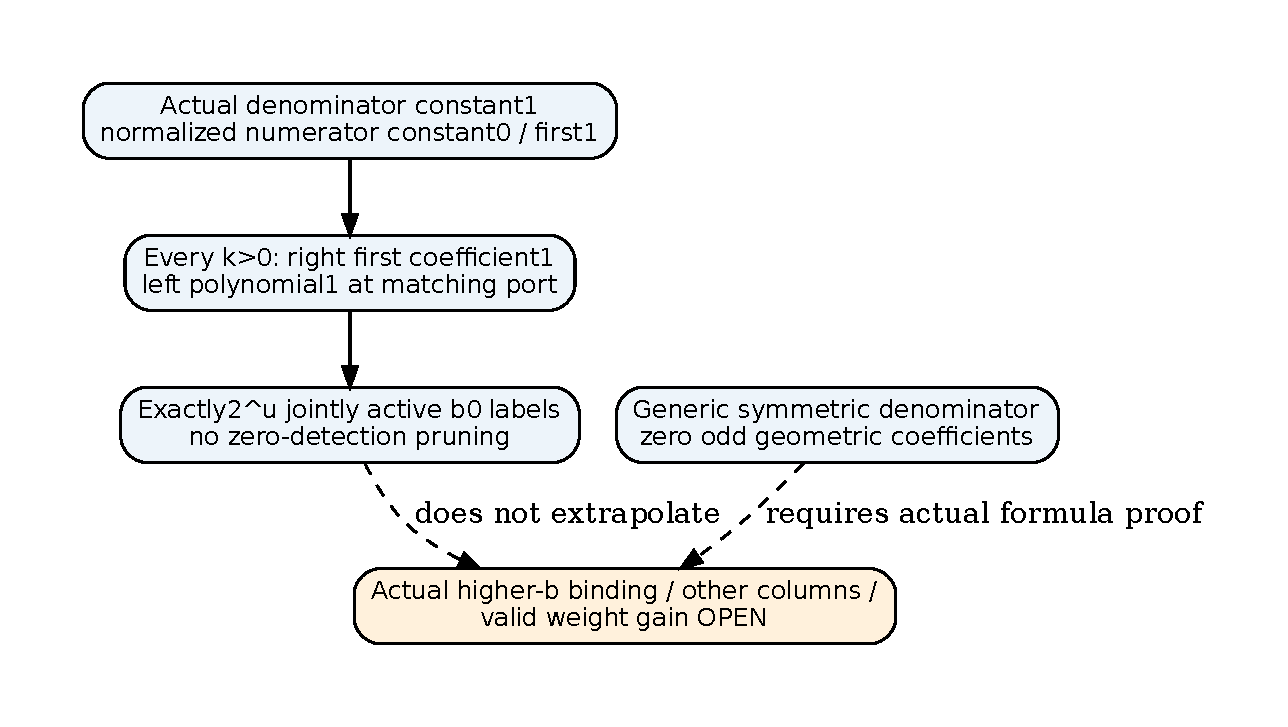
\includegraphics[height=2.8in]{zeroth-allk-dependencies-001.pdf}\end{center}

\textbf{Next discriminating test.} At a negative pole $-2^i$, select a single
retained anchor at $+2^i$ with multiplicity one and other multiplicities zero.
At matching ports, check the actual $Z=0$ denominator against the symmetric
pair. Prove or refute the odd leading-$H$ coefficient cancellation, retaining
positive, zero and empty-cutoff controls. Then test other columns and higher
coefficients before deriving any valid mode-weight improvement. Do not use
this generic identity as an assumed support-pruning rule [pcc:unverified].

\textbf{Remaining interfaces.} Every declared $2^u k$ label stays charged
until actual support or valuation improvements are proved. Original packet
metadata and child budgets, complete scalar/AST/denominator/encoding/control/
array/index/trace/memory costs, actual elliptic relation, public finder,
field/scalar extraction, retries and full expected bit cost remain open.
The PR watcher remains paused, and protected history is untouched. No
native timing, scaling, paid/cloud or attack campaign was launched
[pcc:unverified].
\end{document}
